% \begin{figure}[!htb]
% \centering
% 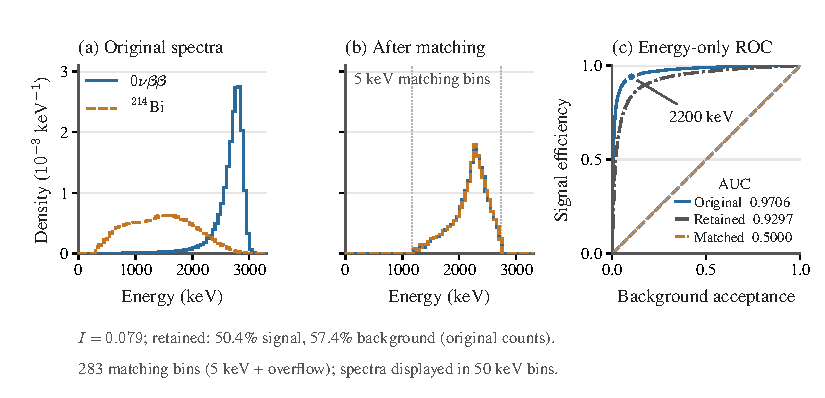
\includegraphics[width=\linewidth]{wing_contribution/figures/supernemo_energy_matching_auc.pdf}
% \caption{SuperNEMO energy matching and its effect on the fixed score
% $s=E_1+E_2$ for $0\nu\beta\beta$ versus $^{214}$Bi.
% (a,b) Class-normalized energy spectra before and after matching, displayed
% in 50\,keV bins. The original sample contains 196,608 signal and 262,144
% background events. Matching equalizes class mass in 283 valid
% 5\,keV bins from the shared regular-plus-overflow grid and retains 50.4\% and 57.4\% of events, respectively;
% vertical guides in (b) mark the common-support boundaries.
% (c) Original, unweighted retained-population, and matched AUCs are
% 0.9706, 0.9297, and 0.5000. The retained and matched curves use the same
% events after support restriction and sparse-bin exclusion.
% The point marks the 2200\,keV cut on the original population.}
% \label{fig:energybench-auc}
% \end{figure}
